%%%%%%%%%%%%%%%%%%%%%%%%%%%%%%%%%%%%%%%%%%%%%%%%%%%%%%%%%%%%%%%
%
% Introduction.tex (part of thesis.tex)
% author: Qie Hu
%
%%%%%%%%%%%%%%%%%%%%%%%%%%%%%%%%%%%%%%%%%%%%%%%%%%%%%%%%%%%%%%%

%!TEX root = ../../thesis.tex

\section{Experimental Results}\label{sec:results}


%%%%%%%%%%%%%%%%%%%%%%%%%%%%%%%%%%%%%%%%%%%%%%%%%%%
%%%%%%%%%%%%%%%%%%%%%%%%%%%%%%%%%%%%%%%%%%%%%%%%%%%

\subsection{Communication Architecture}\label{sec:comm}

The communication architecture is shown in Figure \ref{fig:comm_architecture}.
The HLC is implemented in Matlab on a standard laptop and the LLC is implemented in Python on a server located in SDH.
The Matlab and Python scripts communicate asynchronously via local port forwarding and TCP/IP.
All requests are initiated from the Matlab script and forwarded to the connected port on the laptop, while the Python script continuously listens to the corresponding port on the server and responds to any received requests.

The HLC queries the publicly available database of \textit{darksky.net} to obtain weather forecasts, and collects building measurements by sending read requests to the Python script, which then directly queries the BACnet to obtain these measurements. 
At the same time, the HLC computes the regulation capacities, baseline and optimal airflow rate setpoints and sends them as write requests to the Python script. The script then updates the values of its local copy of the regulation capacities and baseline, and adjusts the appropriate actuator setpoints via BACnet.
Finally, the LLC reads the preloaded PJM regulation signal, and determines and adjusts the fan speed setpoint using read and write requests via the BACnet.  

\begin{figure}[t]
\centering
%\vspace*{-0.4cm}
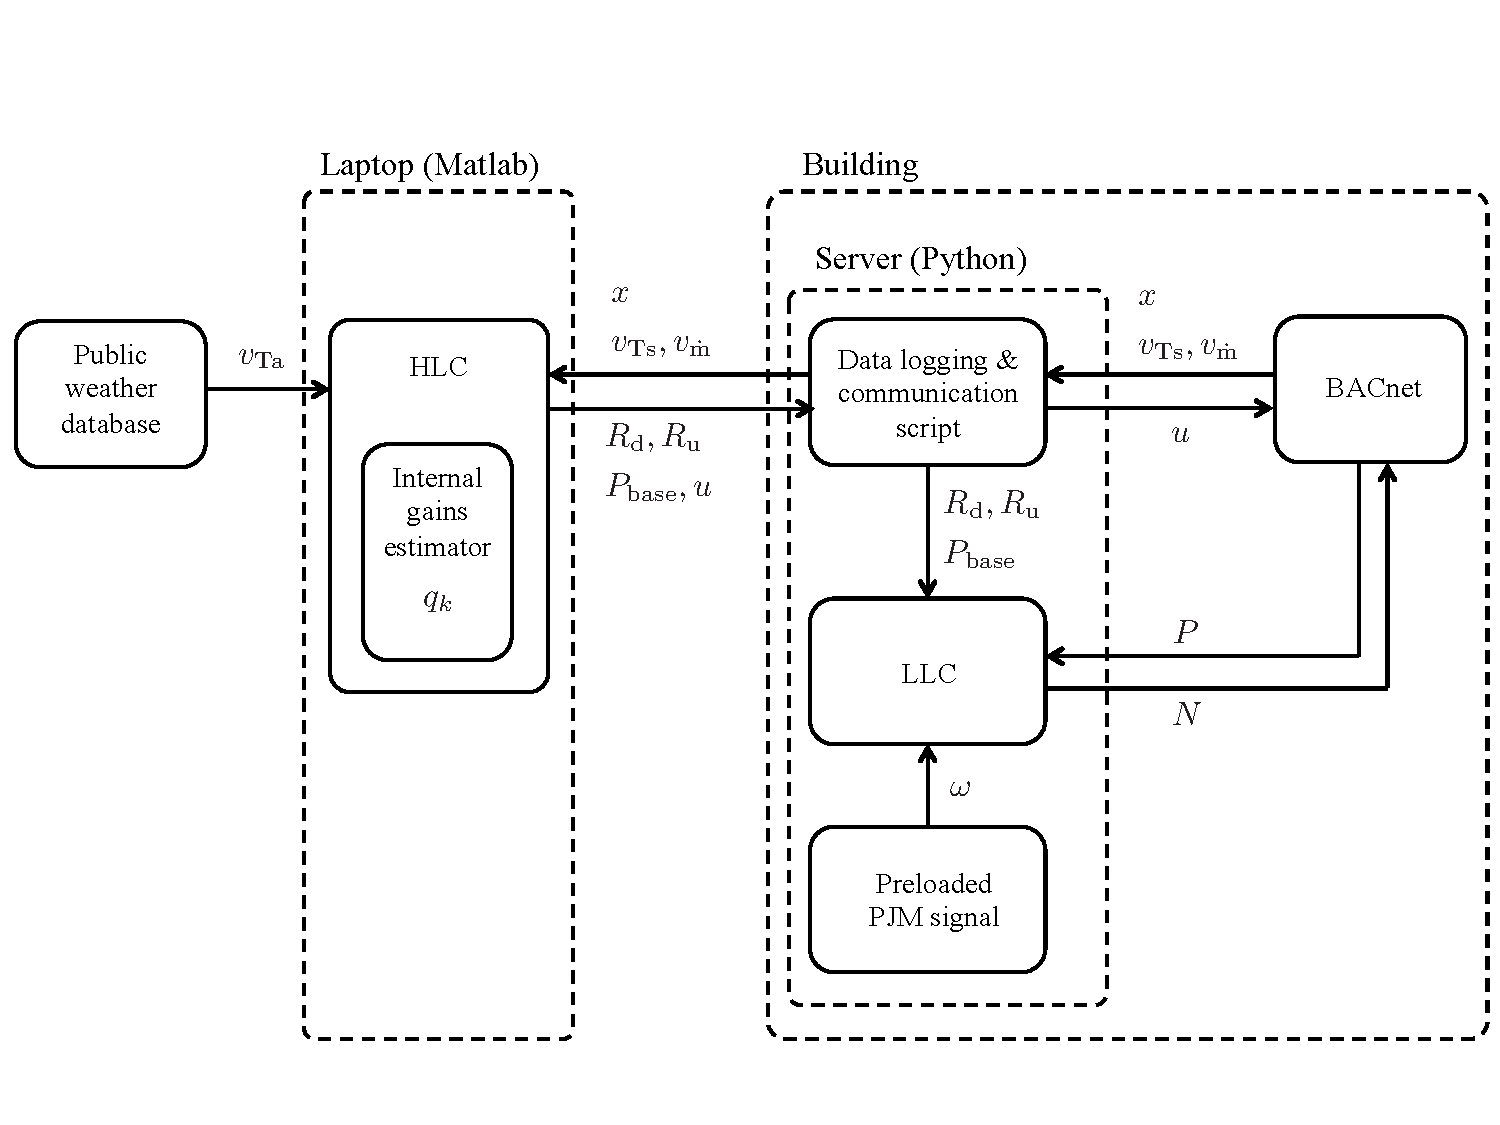
\includegraphics[width = \textwidth]{chapters/building_exp/figures/comm_architecture.pdf}
%\vspace*{-0.5cm}
\caption{Communication architecture. See Table \ref{tab:notation} for description of symbols.}
\label{fig:comm_architecture}
\vspace*{-0.45cm}
\end{figure}


%%%%%%%%%%%%%%%%%%%%%%%%%%%%%%%%%%%%%%%%%%%%%%%%%%%
%%%%%%%%%%%%%%%%%%%%%%%%%%%%%%%%%%%%%%%%%%%%%%%%%%%


\subsection{Performance Metric}\label{sec:performance_metric}

PJM's composite performance score $S_\text{comp}$ is used to evaluate our controller's performance in tracking the regulation signal. 
This score consists of three equally weighted components: a correlation score $S_\text{c}$, a delay score $S_\text{d}$ and a precision score $S_\text{p}$, defined as in \cite{PJM12}:

\begin{equation}\label{eq:pjm_score}
\begin{aligned}
S_\text{c} = & \max_{t \in [0, 5 \text{min}]} (\sigma_t) \\
S_\text{d} = & \frac{1}{5 \text{min}} \left(5 \text{min} - \frac{\max(t^\star - 10 \text{sec},0)}{60\text{sec}}\right) \\
& \text{where}~t^\star =  \arg\max_{t \in [0, 5 \text{min}]} (\sigma_t)\\
S_\text{p} = & 1 - \frac{1}{n_h} \sum_{k=1}^{n_h}  \frac{\left | P_{\text{ref}}(k) - P(k)\right |}{0.5\cdot(R_{\text{d},h} + R_{\text{u},h})}  \\
S_\text{comp} = & \frac{1}{3} \cdot \left( S_\text{c} + S_\text{d} + S_\text{p} \right).\\
\end{aligned}
\end{equation}

In \eqref{eq:pjm_score}, $\sigma_t$ represents the correlation between the reference signal $P_{\text{ref}}(k)$ and the fans' actual power consumption delayed by $t$ seconds $P(k+t)$. 
In other words, $S_\text{c}$ measures the maximum correlation between the regulation signal and the building's response signal within each 5 minute window. $S_\text{d}$ represents the response delay when maximum correlation occurs, with a ``free'' 10 second allowance, and finally $S_\text{p}$ measures the average tracking error scaled by the building's regulation capacity offered for that hour $h$.
All scores take values between 0 and 1, with 1 being a perfect score. 
Following PJM's rule, we generate $S_\text{c}$ and $S_\text{d}$ every 10 seconds and calculate $S_\text{p}$ once per hour.
The performance score $S_\text{comp}$ is then computed every hour by averaging $S_\text{c}$ and $S_\text{d}$ scores for the hour and using $S_\text{p}$ for that hour.



%%%%%%%%%%%%%%%%%%%%%%%%%%%%%%%%%%%%%%%%%%%%%%%%%%%
%%%%%%%%%%%%%%%%%%%%%%%%%%%%%%%%%%%%%%%%%%%%%%%%%%%

\subsection{Certification Experiment}\label{sec:certification_exp}
Any resource that intends to participate in PJM's regulation market must first pass the certification test, which is run during a continuous 40-minute period, using the test signal published on PJM's website \cite{PJM_signal_price}.
The test is scored using $S_\text{comp}$ evaluated on the entire 40-minute test period, and a resource is certified only after it achieves three consecutive scores of 0.75 or above.
In addition, both the baseline consumption and regulation capacity must be declared before the test begins and remain constant throughout the test.

%The resource must set and hold for the test duration the MW-value base point that the resource is regulating around. Changes in base loading for a resource during the test period invalidates the test. Once the test is announced, a resource is not permitted to change its regulation capacity.

%The first of these test may be performed internally by the member following the PJM Regulation test procedure. The remaining tests should be administered by PJM Dispatch.

We carried out four certification tests at various hours of the day from November 27 (Sunday) to 28 (Monday) 2016 and achieved $S_\text{comp}$ values around 0.9 in all tests (Table \ref{tab:certification}). This demonstrates that our controller's performance is robust to disturbances such as weather and occupancy. 
Figure \ref{fig:cert_power} shows the desired reference signal $P_{\text{ref}}$, the fan's actual power consumption $P$ and the percentage tracking error defined as $(P_\text{ref} - P)/P_\text{ref} \cdot 100 $ for the test conducted on November 28 starting at 10~a.m.. An absolute tracking error of less than 28\% is observed during 90\% of the test period.

\begin{table}[b]
\centering
\begin{tabular}{c | c | c c c | c}
\toprule
Test date & Test start time & $S_\text{c}$ & $S_\text{d}$ & $S_\text{p}$ & $S_\text{comp}$  \\ \hline
Nov 27 & 22 hours & 0.90 & 0.90 & 0.88 & 0.89\\
Nov 28 & 10 hours & 0.93 & 0.93 & 0.88 & 0.91 \\
Nov 28 & 13 hours & 0.92 & 0.90 & 0.89 & 0.90 \\
Nov 28 & 16 hours & 0.93 & 0.92 & 0.89 & 0.91 \\
\bottomrule
\end{tabular}
\caption{PJM performance scores for certification tests.}
\label{tab:certification}
\end{table}

\begin{figure}[t]
\centering
%\vspace*{-0.4cm}
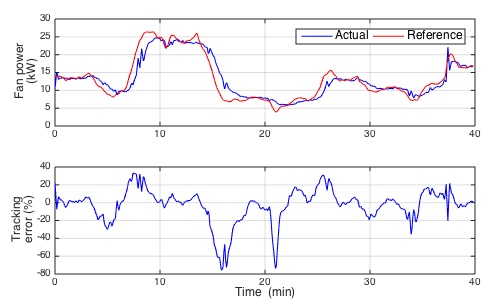
\includegraphics[scale=0.7]{chapters/building_exp/figures/Cert_power.png}
%\vspace*{-0.5cm}
\caption{Certification experiment results: power and tracking error.}
\label{fig:cert_power}
%\vspace*{-0.45cm}
\end{figure}


%%%%%%%%%%%%%%%%%%%%%%%%%%%%%%%%%%%%%%%%%%%%%%%%%%%
%%%%%%%%%%%%%%%%%%%%%%%%%%%%%%%%%%%%%%%%%%%%%%%%%%%

\subsection{Tracking Experiment}\label{sec:tracking_exp}
In this section, we present the results from the tracking experiment conducted from 13:00 to 17:00 on Nov 29, 2016, which uses the historic PJM RegD signal recorded from 13:00 to 17:00 on July 1, 2016 \cite{PJM_signal_price} as the reference frequency regulation signal.

After successful certification, each resource must maintain a historic performance score $S_\text{comp}$ of above 40\% to continue to provide regulation services. In addition, a resource must achieve an average hourly score of at least 50\% to receive payments for offering regulation capacity. 
Table \ref{tab:tracking} shows the $S_\text{comp}$ scores calculated for each hour, as well as the average scores, of our tracking experiment.
Our controller scored $S_\text{comp}$ values well above both thresholds during the field experiment, demonstrating good tracking performance. 

%Regulating resources that have not met performance thresholds over a specified time period will be disqualified and must re-qualify to offer into the regulating market. The disqualification threshold is based on the historic performance score. The historic performance score is a rolling average actual hourly performance score for the last 100 hours a resource has operated. When the historic performance score falls below 40\%, the resource will no longer be eligible to offer into the regulation market.

\begin{table}[b]
\centering
\begin{tabular}{c | c c c | c}
\toprule
 & $S_\text{c}$ & $S_\text{d}$ & $S_\text{p}$ & $S_\text{comp}$  \\ \hline
1\textsuperscript{st} hour & 0.94 & 0.91 & 0.99 & 0.95\\
2\textsuperscript{nd} hour & 0.72 & 0.52 & 0.99 & 0.74 \\
3\textsuperscript{rd} hour & 0.63 & 0.63 & 0.99 & 0.75 \\
4\textsuperscript{th} hour & 0.62 & 0.31 & 0.99 & 0.64 \\ %\hline
Mean & 0.73 & 0.59 & 0.99 & 0.77 \\
\bottomrule
\end{tabular}
\caption{PJM performance scores for tracking experiment.}
\label{tab:tracking}
\end{table}

Figure \ref{fig:track_power} shows that the actual fan power closely tracks the reference power signal and indeed, an absolute tracking error of less than 16\% is achieved 90\% of the time. The error is greatest at the start of the experiment as the fans switch from normal operation to frequency regulation mode, and decays as the experiment progresses.
The fans offer a constant total regulation capacity of 23.3 kW every hour, % This is because the constraints on fan speed (N_min and N_max) are active at the optimal solution, which translates to fixed power difference P(N_max) - P(N_min).
but the split between up- and down-regulation capacities varies hourly as the building's baseline consumption changes. 
Finally, we confirm that the duct static pressure remains below the maximum limit of 2 inches water column throughout the experiment.

We present the zone temperatures and airflow rates from the experiment in Figure \ref{fig:track_temp_flow}, and note the following observations. 
First, all zone temperatures are maintained within the comfort bounds and flow rates are kept within the permissible ranges. 
Second, to minimize electricity cost, flow rates are kept at their minima unless continued supply of minimum airflow to a zone is predicted to cause the zone temperature to exceed its maximum limit within the prediction horizon. 
For example, flow rates are increased in the second and third hours in the West zone to maintain occupant comfort. 
Third, observe that temperatures decrease during the third hour in the West zone and the second hour in the South zone, which indicates that the rooms are overcooled, i.e., supply air's flow rates are more than the minimum required to maintain zone temperatures within the comfort range. 
This is likely due to disturbance prediction errors.

%\textcolor{red}{Comment on power tracking, when is it good/bad, when is PI controller used/feedforward controller used. Room temperatures are not exceeded.}

\begin{figure}[t]
\centering
\vspace*{1cm}
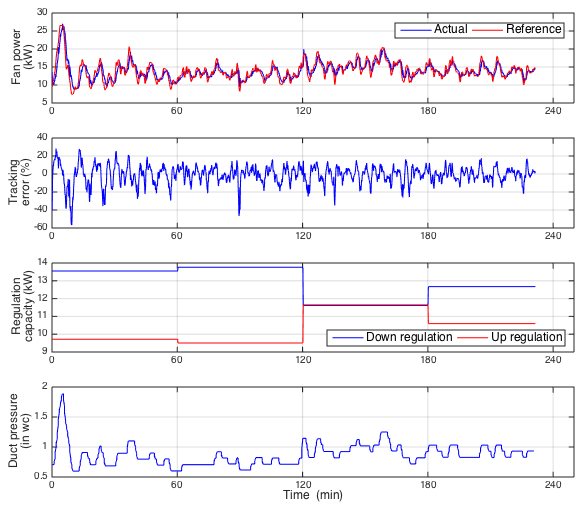
\includegraphics[width=\textwidth]{chapters/building_exp/figures/Track_power.png}
%\vspace*{-0.4cm}
\caption{Tracking experiment results: power, tracking error, regulation capacities and duct pressure.}
\label{fig:track_power}
%\vspace*{-0.45cm}
\end{figure}

\begin{figure}[t]
\centering
%\vspace*{-0.5cm}
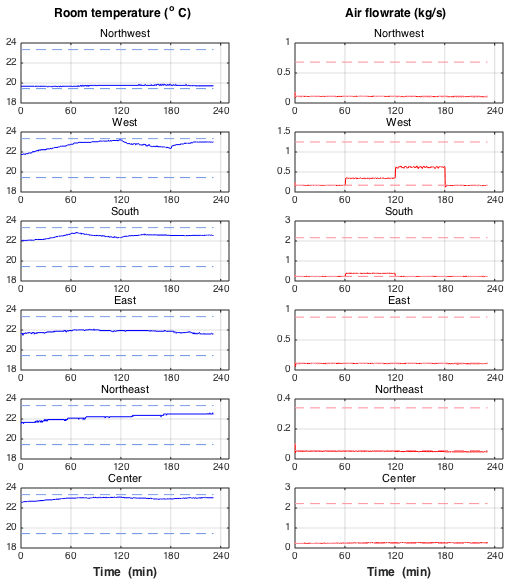
\includegraphics[width=\textwidth]{chapters/building_exp/figures/Track_temp_flow.png}
%\vspace*{-0.9cm}
\caption{Tracking experiment results: room temperatures and airflow rates. Solid lines are actual values, dashed lines are maximum and minimum limits.}
\label{fig:track_temp_flow}
%\vspace*{-0.45cm}
\end{figure}



%%%%%%%%%%%%%%%%%%%%%%%%%%%%%%%%%%%%%%%%%%%%%%%%%%%%
%%%%%%%%%%%%%%%%%%%%%%%%%%%%%%%%%%%%%%%%%%%%%%%%%%%%
%
%\subsection{Economic Potential}\label{sec:eco_potential}
%In this section, we use PJM's publicly available policy manuals \cite{PJM12} and market data \cite{PJM_signal_price} to estimate the revenue that SDH and similar buildings can obtain for offering regulation service.
%The fourth floor provided a regulation capacity of 23.3 kW during its operational hours. 
%%Assuming that each of the seven floors of SDH can provide the same capacity as the fourth floor does, then the entire building can provide 163 kW capacity for frequency regulation. 
%Assuming the building provides regulation service throughout the day, and receives an average reward of \$7.98/MWh, based on PJM's 2016 market data \cite{PJM_signal_price}, then its yearly revenue is estimated to be \$1,630.
%% Divided regulation payment of $15.96 by 2, as payment is for 1MWh of up and down capacity, i.e. +/- 1MWh of capacity (2 MWh total) gets paid $15.96 per hour.


%In this section, we use PJM's publicly available policy manuals \cite{PJM12} and market data \cite{PJM_signal_price} to estimate the revenue that SDH and similar buildings can obtain for offering regulation service.
%The fourth floor provided a regulation capacity of 23.3 kW during its operational hours. 
%Assuming that each of the seven floors of SDH can provide the same capacity as the fourth floor does, then the entire building can provide 163 kW capacity for frequency regulation. 
%Assuming SDH provides regulation service throughout the day, and receives an average reward of \$7.98/MWh, based on PJM's market data for July 2016 \cite{PJM_signal_price}, then its yearly revenue is estimated to be \$11,300.
%% Divided regulation payment of $15.96 by 2, as payment is for 1MWh of up and down capacity, i.e. +/- 1MWh of capacity (2 MWh total) gets paid $15.96 per hour.
%






